% Author: Raphael Champeimont
% This document is in the public domain.
\documentclass[12pt,a4paper]{article}

\setlength{\topmargin}{0mm}      % no margin above heading
\setlength{\parindent}{0mm}      % no paragraph identation
\setlength{\parskip}{4mm}        % skip a line between paragraphs
\setlength{\unitlength}{1mm}

% Paper-saving settings
\setlength{\textwidth}{16cm}     % larger page
\setlength{\oddsidemargin}{0mm}  % no left margin
\setlength{\evensidemargin}{0mm} % the same, on even pages
\setlength{\textheight}{22.5cm}  % longer page

%\usepackage[french]{babel}
\usepackage[utf8]{inputenc}
\usepackage{amsmath}
\usepackage{amsfonts}
\usepackage{amssymb}
\usepackage{amsthm}
%\usepackage{pict2e}
\usepackage{graphicx}
\usepackage{lscape}
\usepackage{url}

\newcommand{\N}{\ensuremath{\mathbb{N}}}
\newcommand{\Z}{\ensuremath{\mathbb{Z}}}
\newcommand{\D}{\ensuremath{\mathbb{D}}}
\newcommand{\Q}{\ensuremath{\mathbb{Q}}}
\newcommand{\R}{\ensuremath{\mathbb{R}}}
\newcommand{\C}{\ensuremath{\mathbb{C}}}
\newcommand{\question}[1]{{\fbox{#1} }}
\newcommand{\Vect}{\mathrm{Vect}}
\newcommand{\exercice}[1]{{\bf Exercice #1 }}
\newcommand{\Id}{\mathrm{Id}}
\newcommand{\im}{\mathrm{Im\,}}
\newcommand{\rsx}[2]{{#1|_{#2}}}
\newcommand{\case}[3]{{#1}_{{#2}{#3}}}
\newcommand{\pgcd}{\mathrm{pgcd}}
\newcommand{\ppcm}{\mathrm{ppcm}}

\title{Hash Functions}
\author{Raphael Champeimont}

\begin{document}

\bibliographystyle{plain}
\nocite{*}

\maketitle

\tableofcontents

\newpage

\section{Introduction}
When sending information, it is often necessary to ensure that data has been successfully transferred and has not been altered. For example, Alice wants to send a file to Bob, so she uploads it to a server. But Bob does not trust the server, and wants to ensure that the file he downloaded from the server is identical to Alice's original. Hash functions are an answer to that sort of problem. Alice and Bob can then both compute a small piece of data called a hash, and compare their hashes, which must match if the copy has not been altered.


\section{Uses and properties of hash functions}
A hash function is a function $f$ that takes a unbounded block of data (thus a infinite number of possibilities), and returns a (usually small) fixed amount of data (a finite number of values). The result of that function is called a {\em hash}. An obvious consequence of this definition is that such a function necessarily has collisions, ie. distinct values $x$ and $y$ such that $f(x)=f(y)$. All the work on hash functions is about the likeliness and difficulty of finding collisions. It should be noted that hash functions are not expected to be private, but are publicly known algorithms.

This definition both applies to cryptographic hash functions and hash functions used to build hash tables. A hash table is a data structure used for fast access to its elements. In the case of hash tables, it is necessary to avoid collisions between elements in the hash table to be as fast as possible, but if a collision occurs it only results in a loss of time. Cryptographic hash functions, on the other hand, want to avoid collisions between bigger sets of data, and it is important for security to avoid collisions. What we will discuss here is cryptographic hash functions only, but we will simply call them ``hash functions''.

We are going to explore different uses of hash functions, and the properties they require from hash functions.



\subsection{Against accidental modification of a file}

A first possible use of a hash function is to serve as a checksum, protecting against errors occurring because of the possible unreliability of the transfer method. Suppose, for instance, that Alice wants to send a file to Bob. She uploads it to his machine. But Bob is unsure whether the file is intact or has been corrupted. A possible solution would be to transfer the file twice and compare the two, but this requires twice as much upload time. Using a hash function provides a better solution. Both Alice and Bob can compute a hash of their files, using the same hash function. A typical hash functions is expected to provide small hashes (usually less that 1 KB), so Alice can send her hash to Bob using a trusted (but which can be slow and limited) means of communication. Then Bob compared his computed hash and the one sent by Alice. If the two match, Bob can reasonably assume that the file has been successfully transferred.

In this situation, we suppose that the threat to the successful transfer of the file is the unreliability of machines. That means that if an error occurs, it will be a random error, not a deliberate attempt to fake the file.

A trivial hash function that would simply take the first 128 bits of the file as a hash would not work, because a random error in any other part of the file would not change the hash. But a simple modular sum, for example the sum of all the bytes of the file, modulo $2^{128}$ (for a 128 bit hash) would work. Changing a random bit of the file would probably yield a different checksum.

\subsubsection{Associated problem: Comparing files}
A problem of the same type is about comparing files. Suppose that Alice and Bob both have a big file and a slow connection. They want to know if they have the same version of a file. Alice could send her file to Bob who would then compare it, but it would be too long to transfer it. The solution is that Alice and Bob both compute a hash of their files, and compare the hash. This situation is similar to the previous integrity problem, because it is about comparing files which have are not specifically written to produce a collision.



\subsection{Against deliberate forgery of a file}
The goal of hash functions is not only to prevent an accidental damage to the data, but also to prevent a deliberate attempt to fake the file. We suppose we still have Alice who wants to send a file $x$ to Bob, using an untrusted server. But Mallory connects to the server and replaces Alice's file (by a virus for example), and knows which hash algorithm Alice and Bob are using. For Alice to believe the file is intact, Mallory needs to produce a file with the same hash as the original. For Alice's security, the hash function should not make this task possible for Mallory.

This property can me stated precisely: For a given $x$, it should be hard to find a distinct $y$ such that $f(x)=f(y)$.

Of course, it cannot be required that it must be impossible, because $f$ cannot be injective. Mallory could still try many random files and compute their hashes, until he finds one with the same hash as $x$, but this would take a very long time (more than Mallory's life for example) or would require Mallory to be extremely lucky.

The proposed modular checksum of the previous section would not satisfy this property, because it is easy to modify a file and predict in which way it will change the sum. If Alice and Bob use a modular sum, Mallory could create a virus, then write a big comment at the end, filled with garbage so that the sum equals $f(x)$. It is easy for Mallory to know what to write in the comment if the hash function is simply a sum. Therefore, to satisfy this property, we must be cleverer when designing a hash function.

\subsection{Storing passwords}
Another use of hash functions is to store passwords. A server might store a list of logins and passwords in clear, but this requires the password database to be absolutely secret. A improved security would be to store the password hashes instead of the passwords themselves. Suppose Alice defines a new password, the server them computes its hash using a defined hash function. The hash is stored in the password database. Then, when Alice wants to log in, she enters her password. The server then computes the hash of the entered password and compares it to the one in the database. If they don't match, the entered password is wrong. If they match, the entered password is (almost certainly) correct.

Why is this an additional security? Because if Mallory succeeds in reading the password file, he won't be able to know the users' passwords. For that to be impossible (or at least not easily possible), the hash function must be one-way, ie. it must be impossible (in a reasonable time)  given a hash $y$ to compute an $x$ such that $y=f(x)$.

It should be noted that this requirement on the hash function is weaker that the one about integrity of files, because in that previous problem, the attacker was excepted to know an $x$ such that $y=f(x)$ and tried to find a $x'\neq x$ such that $y=f(x')$. In the password case, the attacker only knows $y$. In fact, in a subsequent section, we are going to see that we would like the hash function to have en ever stronger property than these two.

\subsection{Digital signature}
In these modern ages, there is a need for {\em signing} digital documents. On a paper, a signature is something that proves that a document was read and accepted by someone, or was written by that person. It is expected that a signature is something that is unique to a person and that {\em only him} can write.

There is a similar concept for digital documents. We suppose that Alice keeps secret a injective function $g$ but gives $g^{-1}$ to the public. She wants to sign Bob's contract. She can do the following: First, she computes the hash of a the contract $C$ using a publicly known hash function $f$. Then she applies her $g$ function to $f(C)$. She finally adds $g(f(C))$ at the end of the contract. This added text is the signature. She then sends the contract to Bob. Bob can check and prove that Alice did sign the contract, by doing the following: He computes $f(C)$ using the hash function. Then he reads the signature $s$, and computes $g^{-1}(s)$. If $s$ is Alice's signature on contract $C$, then we have $s=g(f(C))$. Therefore
\[ g^{-1}(s) = g^{-1}(g(f(C))) = f(C) \]
Bob can then compare $f(C)$ with $g^{-1}(s)$, which will match if Alice signed the contract. As we can see, the signature $s=g(f(C))$ can only be computed by Alice (her secret $g$ function) and is specific to the $C$ contract (one cannot copy Alice's signature on a contract an put it on an other contract).

In practice, the $g$ function is an encryption algorithm with a private key, while $g^{-1}$ is the associated decryption algorithm with the corresponding public key. See figure \ref{fig:dsd}.

\begin{figure}[h]
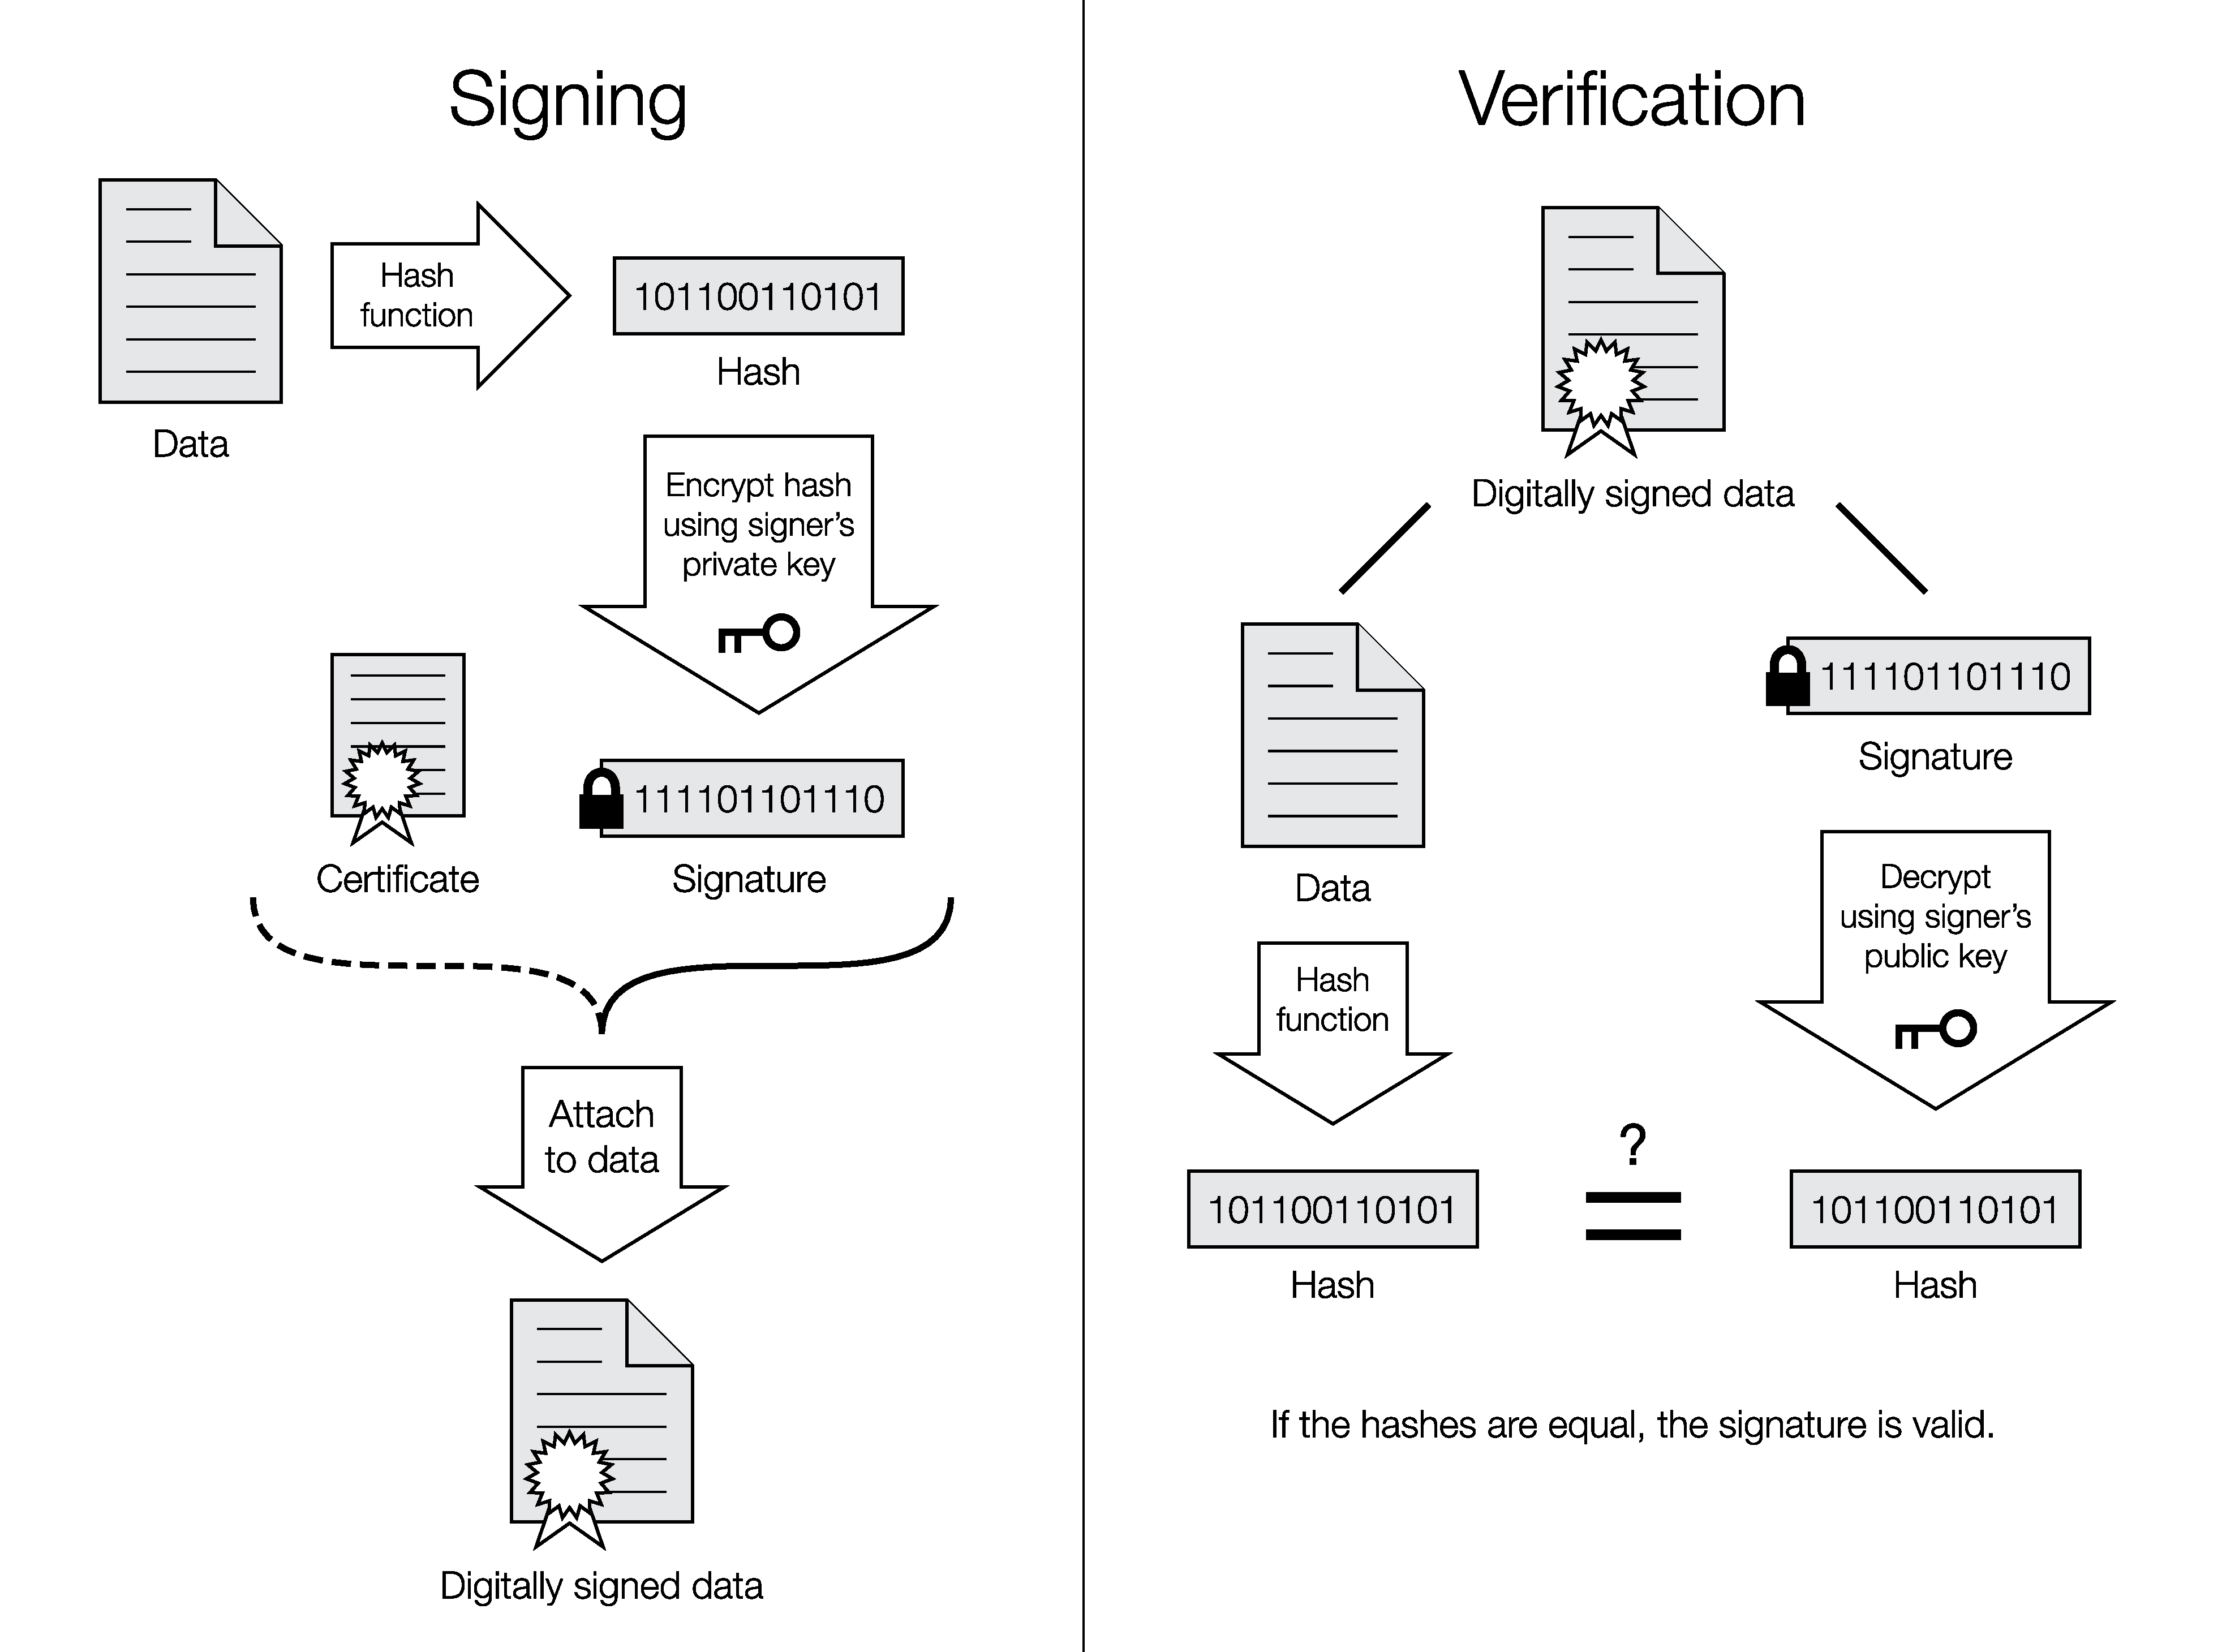
\includegraphics[width=16cm]{Digital_Signature_diagram.pdf}
\caption{Use of hash functions in digital signing. Source: Wikipedia}\label{fig:dsd}
\end{figure}

\subsection{Birthday attack}

\subsubsection{Definition}

In the case where Mallory wants, given a message $x$, to find an $y$ such that $f(x)=f(y)$, an obvious way to proceed is a brute force attack. He can try every possible string $y$ and compute its hash until it matches $f(x)$. Therefore, in the previous sections, we required it to be difficult to do that. But we could require a stronger property: It should be hard to find an $x$ and a (different) $y$ such that $f(x)=f(y)$.

\subsubsection{A probability problem}

We might wonder whether this is really a stronger requirement. Consider the following situation: You are in a room with 57 people. What is the probability that one of them has his birthday the same day as you? It is only $14\%$. But what is now the probability that there are two people in that room with their birthday the same day? It is $99\%$. This is called the {\em birthday problem}.

In the case of hash functions, the birthday problem means that it is a lot faster to find a couple $(x,y)$ such that $f(x)=f(y)$ than, for a given $x$, to find an $y$ such that $f(x)=f(y)$ (assuming that every hash is equally probable). More precisely, if the number of possible hashes is $n$, you can expect to find a collision after $1.25 \sqrt{n}$ tryouts in the case of a $(x,y)$ couple, while you need to do $0.5 n$ tryouts if $x$ is fixed. Trying to find such an $(x,y)$ couple is called a {\em birthday attack}.

\subsubsection{A possible birthday attack}

This sort of attack might be used the following way: Mallory wants to trick Alice into signing a fraudulent contract. He writes a fair contract $x_0$ and a fraudulent one $y_0$. He then computes many variants $x_1, x_2, \ldots, x_n$ of $x_0$ which have the same meaning but differ on small details (presentation, replacing synonyms, etc.). He does the same with $y_0$. Then (or simultaneously) he computes the hashes of all these $x_i$ and $y_i$. Then, for every couple $(i,j)$, he checks whether $f(x_i)=f(y_j)$. This will almost all the time be false, but after some time he may find such a couple $(x_i,y_j)$. He can then send the fair contract $x_i$ to Alice, who will accept to sign it. She then sends back $x_i$ with her signature $s=g(f(x_i))$ (see previous section about digital signing). Mallory then detaches $s$ from $x_i$ and puts it at the end of $y_j$. He then tells Bob that Alice signed his contract $y_j$. Bob wants to see if this is true, so he computes $f(y_j)$ and $g^{-1}(s)$. We have
\[ g^{-1}(s) = g^{-1}(g(f(x_i))) = f(x_i) \]
But, we have $f(x_i)=f(y_j)$, therefore, Bob will find that $g^{-1}(s) = f(y_j)$, and conclude that Alice (almost certainly) signed $y_j$. Alice will then appear to have signed the fraudulent contract $y_j$.

This sort of attack can be applied to all problems of digital signing, like e-mail signing and program signing.

\subsubsection{Solution}

To avoid this problem, it must be too long to do what Mallory has done, ie. compute hashes of many $(x_i,y_j)$ until he finds a collision. The consequence of that is we need to have a number of possible hashes higher (twice as long) that we would have thought if we didn't take in account birthday attacks.

\section{Functions used in the real world}

The two most widely used cryptographic hash functions are MD5 and SHA-1.

\subsection{MD5}

Message-Digest algorithm 5 (MD5) is a widely used hash function, designed by Ron Rivest (who is also one of the three cryptographers who discovered RSA). It was designed in 1991 to replace the MD4 function, which was considered insecure.

\subsubsection{Algorithm}

The MD5 algorithm has 4 global variables, $A$, $B$, $C$, $D$ which are 32-bit integers. First the function cuts the file into 512 bits chunks, padding it if necessary so that its length becomes a multiple of 512.  For each 512-bits chunk, it then runs 64 times a loop. The MD5 algorithm has 4 versions of a function $F$, and changes of $F$ every 16 times. These four $F$ functions are:
\[
\begin{array}{l}
    F(X,Y,Z) = (X\wedge{Y}) \vee (\neg{X} \wedge{Z}) \\
    G(X,Y,Z) = (X\wedge{Z}) \vee (Y \wedge \neg{Z}) \\
    H(X,Y,Z) = X \oplus Y \oplus Z \\
    I(X,Y,Z) = Y \oplus (X \vee \neg{Z}) 
\end{array}
\]
$\oplus, \wedge, \vee, \neg$ denote the bitwise XOR, AND, OR and NOT operations respectively.

The algorithm computes $A + F(B,C,D)$, then adds it to a block of the input file, then adds a constant, rotates the number of 5 bits, and adds $B$. The result of that is the new value of $B$. The new value of $A$ is the old value of $D$, the new value of $C$ is the old value of $B$ and the new value of $D$ is the old value of $C$.

Then it does again that step with the new values of $A$, $B$, $C$, $D$. When it arrives at the end of the input file, it returns the concatenation of these 4 variables, and this is the hash.

\begin{figure}[h]
\begin{center}
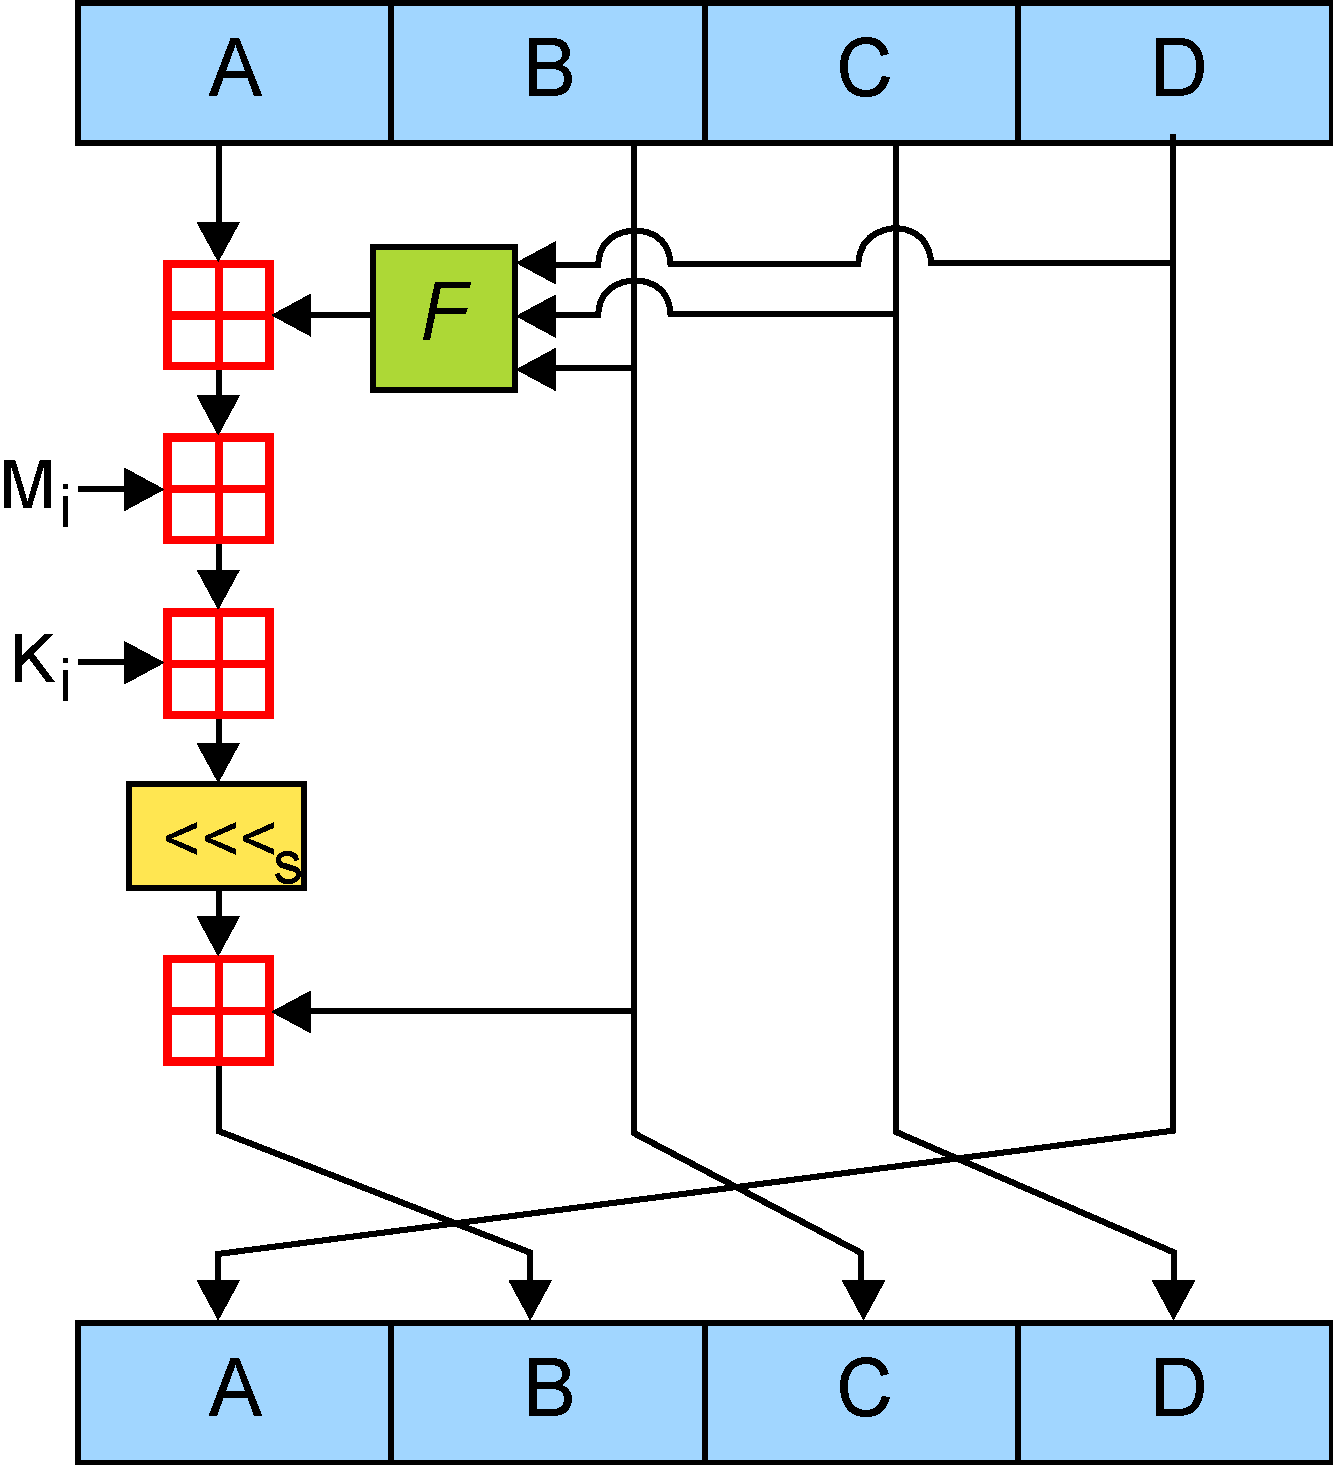
\includegraphics[width=7cm]{MD5.pdf}
\end{center}
\caption{A diagram showing one MD5 operation. The red pluses in squares are additions modulo $2^{32}$, $M_i$ is a piece of the input file and $K_i$ is a constant. Source: Wikipedia}\label{fig:md5}
\end{figure}

\subsubsection{Discovered weaknesses}
In 1995, a theoretical weakness was discovered in MD5. In 2005, researchers successfully made 2 documents with the same MD5 hash. Ron Rivest then said that "md5 and sha1 are both clearly broken (in terms of collision-resistance)". In 2008, the MD5 weakness was used to create a forged SSL certificate.

After that, many companies stopped using MD5. VeriSign (an issuer of SSL certificates) then decided to stop providing MD5-based certificates and moved to the SHA family only. The MD5 algorithm was deprecated by SSL researchers and the US Department of Homeland Security. In a general way, MD5 is now deprecated for all uses in favor of the SHA family.

\subsection{SHA-0 and SHA-1}
Secure Hash Algorithm (SHA) is a family of hash functions written by the NSA (US National Security Agency). The first version (SHA-0) was published in 1993.

\subsubsection{Algorithm}
The general shape of the algorithm is the same as MD5. The input is divided in fixed-length blocks. The algorithm also has a state, and for every block, a new state is computed from the previous state and the read block.

\subsubsection{Discovered weaknesses in SHA-0}
Before the release of SHA-1, an earlier function, SHA-0 was released in 1993. However, it was withdrawn by the NSA, which replaced it by a modified version in 1995: SHA-1. The NSA said that SHA-0 was broken but did not explain why. In 1998, two French researchers discovered what the problem with SHA-0 was, and published the explanation. In 2004, near-collisions were found for SHA-0. Today, it is possible to find a SHA-0 collision in $2^{39}$ operations instead of the expected $2^{80}$.

\subsubsection{Discovered weaknesses in SHA-1}
The SHA-0 function was almost never used, because it was quickly withdrawn and replaced by SHA-1. But as SHA-0 and SHA-1 are very similar, problems found with SHA-0 were also potential problems with SHA-1.

In early 2005, an attack on SHA-1 was published. But only 53 of the 80 rounds were broken.

In February 2005, an other attack was announced. It could find collisions in the full version of SHA-1, requiring fewer than 269 operations. (A brute-force search would require 280 operations.) After that, the NIST (US National Institute of Standards and Technology) planned to phase out the use of SHA-1 in favor of SHA-2.

On 17 August 2005, an improvement on the SHA-1 attack was announced, lowering the complexity required for finding a collision in SHA-1 to 263.

In 2006, a two-block collision for 64-round SHA-1 was presented, found using unoptimized methods with 235 compression function evaluations. As this attack requires the equivalent of about 235 evaluations, it is considered to be a significant theoretical break. In order to find an actual collision in the full 80 rounds of the hash function, however, massive amounts of computer time are required. To that end, a collision search for SHA-1 using the distributed computing platform BOINC began in August 2007 but the effort was abandoned in 2009 due to lack of progress.


\subsection{SHA-2}
The SHA-2 name is a group of four algorithms: SHA-224, SHA-256, SHA-384, and SHA-512. The number represents the number of bits in the hash. These algorithms were published in 2001.

\subsubsection{Discovered weaknesses in SHA-2}

There are two meet-in-the-middle preimage attacks against SHA-2 with a reduced number of rounds. The first one attacks 41-round SHA-256 out of 64 rounds with time complexity of $2^{253.5}$ and space complexity of $2^{16}$, and 46-round SHA-512 out of 80 rounds with time $2^{511.5}$ and space $2^3$. The second one attacks 42-round SHA-256 with time complexity of $2^{251.7}$ and space complexity of $2^{12}$, and 42-round SHA-512 with time $2^{502}$ and space $2^{22}$.

Although these are theoretical weaknesses found on SHA-2, it is not feasible with today's computers to compute a collision.

\subsection{The future: SHA-3}
In order to find a better function than SHA-1 and SHA-2, the NIST launched an open competition in 2007.

In the list of candidates registered in 2008, NIST rejected a lot of them because they were not secure enough. On July 24, 2009, the NIST published the list of 14 candidates that are accepted for round 2. The announcement of the final round is expected for 2010, while the proclamation of the winner is scheduled for 2012.

\section{Conclusion}
Because they are used in file integrity verification and digital signatures, hash functions are a key security feature. Although hash functions are less studied than encryption functions, important progress has been made on them. But many programs still use broken algorithms like MD5, which should always be avoided (except as a checksum against accidental errors). The SHA-1 function is a good compromise between practical security and availability of implementation. If compatibility is a concern (for SSL certificates for example), SHA-2 may not be available on all platforms. However, when designing a new program, the SHA-2 family should be preferred because it represents the best (although not perfect) hash functions available today.





\bibliography{hash_functions}

\end{document}
